%% start of file `template.tex'.
%% Copyright 2006-2013 Xavier Danaux (xdanaux@gmail.com).
%
% This work may be distributed and/or modified under the
% conditions of the LaTeX Project Public License version 1.3c,
% available at http://www.latex-project.org/lppl/.


\documentclass[11pt,a4paper,sans,norsk]{moderncv}        % possible options include font size ('10pt', '11pt' and '12pt'), paper size ('a4paper', 'letterpaper', 'a5paper', 'legalpaper', 'executivepaper' and 'landscape') and font family ('sans' and 'roman')

% modern themes
\moderncvstyle{banking}                            % style options are 'casual' (default), 'classic', 'oldstyle' and 'banking'
\moderncvcolor{blue}                                % color options 'blue' (default), 'orange', 'green', 'red', 'purple', 'grey' and 'black'
%\renewcommand{\familydefault}{\sfdefault}         % to set the default font; use '\sfdefault' for the default sans serif font, '\rmdefault' for the default roman one, or any tex font name
%\nopagenumbers{}                                  % uncomment to suppress automatic page numbering for CVs longer than one page

% character encoding
\usepackage[utf8]{inputenc}                       % if you are not using xelatex ou lualatex, replace by the encoding you are using
%\usepackage{CJKutf8}                              % if you need to use CJK to typeset your resume in Chinese, Japanese or Korean

% adjust the page margins
\usepackage[scale=0.75]{geometry}
%\setlength{\hintscolumnwidth}{3cm}                % if you want to change the width of the column with the dates
%\setlength{\makecvtitlenamewidth}{10cm}           % for the 'classic' style, if you want to force the width allocated to your name and avoid line breaks. be careful though, the length is normally calculated to avoid any overlap with your personal info; use this at your own typographical risks...
\usepackage{mdframed,graphicx,xcolor}
%\usepackage{tikz}
\usepackage{chemstyle}

\usepackage[final]{pdfpages}


\usepackage{import}

\usepackage[norsk]{babel}

% personal data
\name{Anders}{Østevik}
\title{Curriculum Vitae}                               % optional, remove / comment the line if not wanted
%\address{Fantoftveien 14L, PB 1267, 5075 BERGEN}{}{}% optional, remove / comment the line if not wanted; the "postcode city" and and "country" arguments can be omitted or provided empty
%\phone[mobile]{+47 984 92 338}                   % optional, remove / comment the line if not wanted
%\phone[fixed]{01234 123456}                    % optional, remove / comment the line if not wanted
%\phone[fax]{+3~(456)~789~012}                      % optional, remove / comment the line if not wanted
%\email{anders.ostevik91@gmail.com}                               % optional, remove / comment the line if not wanted
%\homepage{www.myname.webs.com}                         % optional, remove / comment the line if not wanted
%\extrainfo{additional information}                 % optional, remove / comment the line if not wanted
%\photo[70pt][0.4pt]{profil}                       % optional, remove / comment the line if not wanted; '64pt' is the height the picture must be resized to, 0.4pt is the thickness of the frame around it (put it to 0pt for no frame) and 'picture' is the name of the picture file
%\quote{Some quote}                                 % optional, remove / comment the line if not wanted

% to show numerical labels in the bibliography (default is to show no labels); only useful if you make citations in your resume
%\makeatletter
%\renewcommand*{\bibliographyitemlabel}{\@biblabel{\arabic{enumiv}}}
%\makeatother
%\renewcommand*{\bibliographyitemlabel}{[\arabic{enumiv}]}% CONSIDER REPLACING THE ABOVE BY THIS

% bibliography with mutiple entries
%\usepackage{multibib}
%\newcites{book,misc}{{Books},{Others}}
%----------------------------------------------------------------------------------
%            content
%----------------------------------------------------------------------------------
\begin{document}
%\begin{CJK*}{UTF8}{gbsn}                          % to typeset your resume in Chinese using CJK
%-----       resume       ---------------------------------------------------------
\makecvtitle

\small{Elektronikkingeniør med bachelor i elektronikk fra Høgskolen i Bergen. Arbeider for øyeblikket med min masteroppgave i fysikk ved Universitetet i Bergen.}

\section{Personlig informasjon}

\begin{minipage}{0.45\textwidth}
	{\renewcommand\labelitemi{}
	\begin{itemize}
	%\item{\textbf{Navn:}	Anders Østevik}
	\vspace{3pt}
	\item{\textbf{Fødselsdato:}	04-07-1991}
	\vspace{3pt}
	\item{\textbf{Kjønn:}	Mann}
	\vspace{3pt}
	\item{\textbf{Adresse:}	Fantoftveien 14L, PB 1267}
	\vspace{3pt}
	\item{\textbf{Postnummer:}	5075 BERGEN}
	\vspace{3pt}
	\item{\textbf{Status:}	Samboer, ingen barn}
	\vspace{3pt}
	\item{\textbf{Mobil:}	+47 984 92 338}
	\vspace{3pt}
	\item{\textbf{Email:}	anders.ostevik91@gmail.com}

	\end{itemize}
	}
\end{minipage} \hfill
\begin{minipage}{0.85\textwidth}
	\begin{figure}[H]
	\setlength{\fboxsep}{1pt}
	\setlength{\fboxrule}{0.1pt}
	\fcolorbox{blue!10}{white!10}{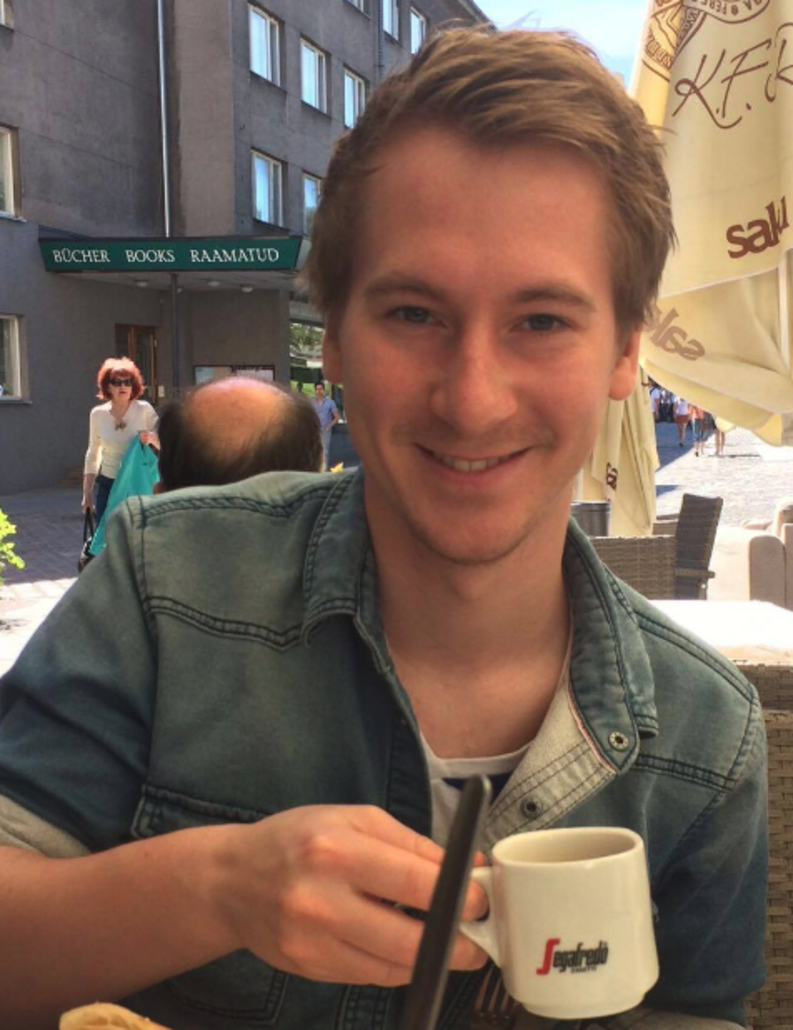
\includegraphics[width=3cm,height=4cm]{profil.pdf}}
	\end{figure}
\end{minipage}

\vspace{6pt}

\section{Utdanning}

\vspace{5pt}

\subsection{Akademiske kvalifikasjoner}

\vspace{5pt}

\begin{itemize}

\item{\cventry{August 2014-- Juni 2016}{Master i Fysikk}{Universitetet i Bergen}{Bergen}{\textit{Mikroelektronikk}}{Analog og digital integrert kretsteknologi, Datamaskinassistert konstruksjon og produksjon av elektronikk, Databehandling i fysikk.}}
\item{\cventry{August 2011-- Juni 2014}{Bachelor i Elektronikk}{Høgskolen i Bergen}{Bergen}{}{Analog krets- og instrumentkonstruksjon, Audioforsterkere, Digitale system (FPGA/VHDL), HW/SW systemkonstruksjon, Digital signalbehandling, Lineære systemer.}}
\item{\cventry{August 2010-- Mai 2011}{Musikk}{Jæren Folkehøgskole}{Jæren}{}{}}
\item{\cventry{August 2007-- Juni 2010}{Studiespesialisering med realfag}{Kopervik Videregående Skole}{Karmøy}{}{}}

\end{itemize}

\vspace{2pt}

\subsection{Større Prosjekter}

\vspace{5pt}

\begin{itemize}

\item{\textbf{Masteroppgave (Pågående):} \textit{'Interface Design for the Gigabit Transceiver Common Readout Unit'}

%\vspace{3pt}

%\small{Selvstendig arbeid over en periode på to semester. Oppgaven gikk ut på å ta del i utviklingen av firmware for en Common Readout Unit (CRU), et utleserkort som skal motta og behandle data fra SLHC (Super Large Hadron Collider), som er i utvikling hos Cern. Oppgaven min fokuserte på seriell kommunikasjon mellom PC og CRU, og PCB design for høyhastighets-transceivere. Oppgaven krevde fordypning i programmeringspråk som C og VHDL, høyhastighets PCB design, testoppsett for forskjellige forsøk (som blant annet innvolverte måling av signalintegritet), og strukturert skriving med gode kunnskaper i engelsk. Av oppgaven har jeg lært å arbeide strukturert, både selvstending og i samarbeid med andre innvolverte i samme prosjekt, der iblant veileder, en doktorgradstudent og en overingeniør. Jeg har blitt mer erfaren med dokumentering av logg, arbeidsliste og rapporter for gjennomført arbeid.}}
}
\vspace{6pt}
%\newpage

\item{\textbf{Bacheloroppgave:} \textit{'Testjigg for ClampOn DSP II Strømforsyningskort'}

%\vspace{3pt}

%\small{Arbeid i gruppe på tre personer over en periode på ett semester. Oppgaven var i samarbeid med bedriften ClampOn og gikk ut på å lage et testoppsett (en såkalt testjigg) for et strømforsyningskort, utviklet av ClampOn. Oppgaven krevde tett samarbeid både med bedrift og internt i gruppen. Oppgaven krevde fordypning i måleteknikk vha. analog og digital elektronikk, programmering av mikrokontrollere og kretsutlegg. Av oppgaven har jeg lært å arbeide effektivt i grupper, å fordele oppgaver jevnt og rettferdig gjennom semesteret, og dokumentering av timelister og rapporter samt generell dokumentering av gjennomført arbeid.}}
}
\end{itemize}

%\newpage

\section{Kurs}
\begin{itemize}
\item{\cventry{Juni 2015}{Todagers kurs i S-parametre med Eric Bogatin}{Practical S-parameter Measurement and Analysis}{København, Danmark}{}{}}
\end{itemize}

\newpage

\section{Arbeidserfaing}

\vspace{6pt}

\begin{itemize}

\item{\cventry{Juni--Juli 2014, Juni--Juli 2012, Juni--August 2011}{Resepsjonist}{Skudenes Legesenter}{Skudeneshavn, Karmøy}{}{\vspace{3pt}Organisering av timelister, pasienttimer, e-resepter og journalutskrifter.}}

\vspace{6pt}

\item{\cventry{Juni--August 2013}{Montør}{Rental Technology \& Service AS}{Åkra, Karmøy}{}{\vspace{3pt}Produksjon og montering
av elektromekaniske komponenter og ulike kabelsett for testing av utstyr.}}

\vspace{6pt}

\item{\cventry{Februar--Mai 2013}{Studieassistent i faget ELE102 Datateknikk}{Høgskolen i Bergen}{Bergen}{}{\vspace{3pt}Studiehjelp med ansvar for retting av innleveringer som omhandlet programmering av mikrokontrollere.}}

\vspace{6pt}

\item{\cventry{Juni--Juli 2009}{Ferievikar}{Karmøy Kommune, parkavdeling}{Skudeneshavn, Karmøy}{}{\vspace{3pt}Diverse oppgaver.}}

\end{itemize}

\section{Tekniske og personlige ferdigheter}

\vspace{6pt}

\begin{itemize}

\item \textbf{Programmingspråk:} Dyktig i: C, C++, Arduino, Avr, TeX, VHDL. \\ Også grunnleggende evner i: Python, C\#, ROOT, SDL, ncurses, Matlab.

\vspace{6pt}

\item \textbf{Software:} Matlab, Labview, LTspice, Cadence, Quartus II, Visual Studio 2010, Microsoft Office.

\vspace{6pt}

\item \textbf{Generelt:} Jobber bra i team, så vel som selvstendig, Er imøtekommende, åpen og utadvendt.

\vspace{6pt}

\item \textbf{Språk:} Snakker og skriver flytende norsk og engelsk.

\vspace{6pt}

\item \textbf{Andre:} Gode ferdigheter innen lodding av komponenter, Evner til å skrive organiserte og strukturerte rapporter, Har førerkort klasse B.

\end{itemize}

%\newpage

\section{Interesser og utemonfaglige aktiviteter}

\vspace{6pt}

\begin{itemize}

\item{Spillprogrammering og 3D-utvikling.}

\vspace{6pt}

\item{Musikk og instrumenter. Jeg har spilt gitar i snart 8 år, selvlært.}

\vspace{6pt}

\item{Småprosjekter med bruk av treverk}

%\vspace{6pt}

%\item{Jeg er også interesert i matlaging, og har en generelt sunn livsstil.}

\end{itemize}

%\section{Referanser}

%\vspace{6pt}
 
%\begin{itemize}

%\item{Ta kontakt.}

%\item{Tone Thorshaug, tidligere Bioingeniør hos Skudenes Legesenter.	(Tlf.: 464 51 589)}
%\item{Attest fra Rental Technology \& Services AS, se vedlegg.}

%\end{itemize}

\vspace{12pt}

\center{Ta gjerne kontakt for mer informasjon.}

%\newpage

%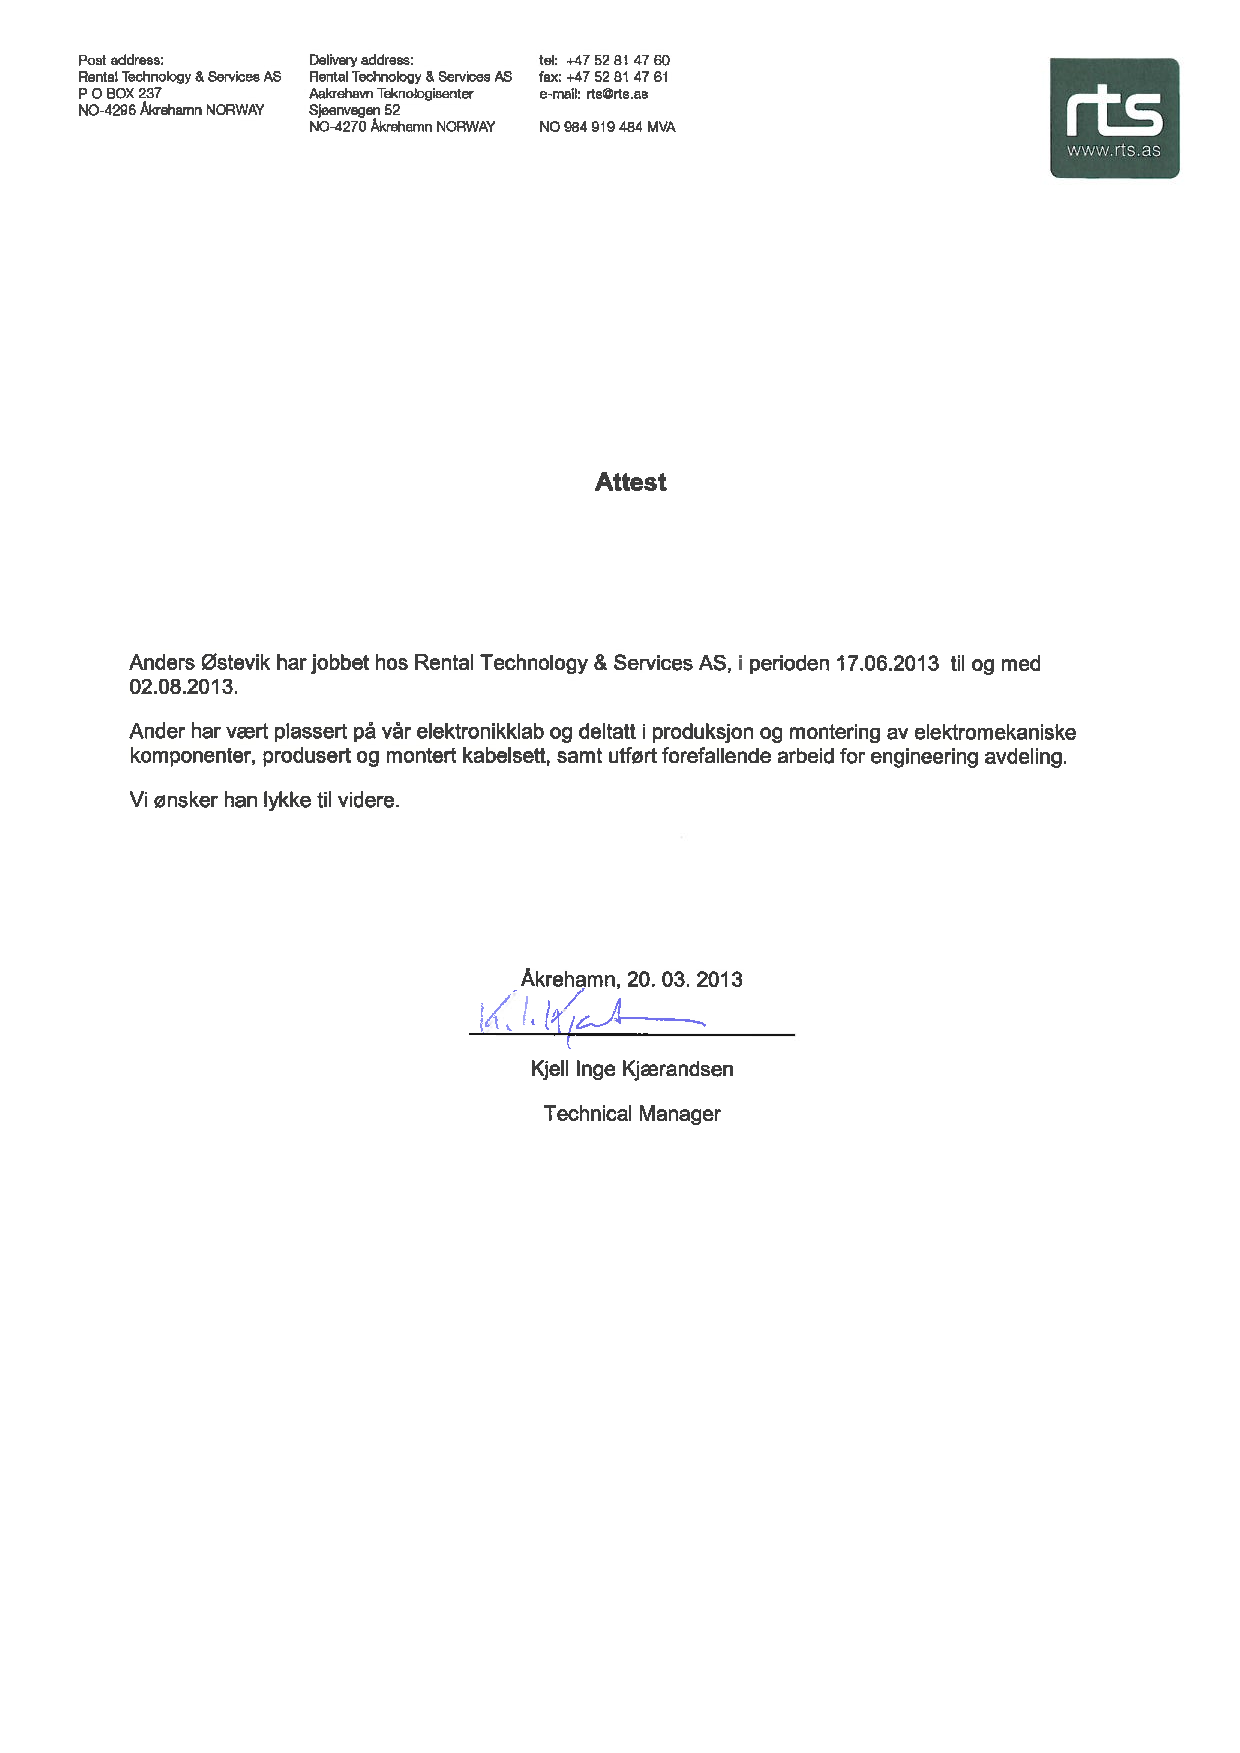
\includepdf[pages=-]{rts.pdf}


\end{document}


%% end of file `template.tex'.
